\begin{table}
\begin{center}
\Large
文档历史发放及记录\vspace{3ex}\\
\scriptsize
\begin{tabular}{|c|c|c|c|c|c|}
\hline
序号 & 变更(+/-说明) & 作者 & 版本号 & 日期 & 批准 \\
\hline  
1 & 创建 & 苏争光 & V0.1 & 2018/8/21 &  \\\hline  
2 & 补充(AM应用内存优化) & 谢杰斌 & V0.2 & 2018/8/27 &  \\\hline
3 & 修改(添加优化概览) & 苏争光 & V0.3 & 2018/8/29 &  \\\hline
4 & 修改(修改AM回收内存机制、应用权限设置) & 张震 & V0.4 & 2018/9/20 &  \\\hline
5 & 修改(添加android进程优先级对比,修改AM进程优先级) & 张震 & V0.5 & 2018/10/12 &  \\
\hline
\end{tabular}
\end{center}
\end{table}
\clearpage

%---------------------------------------------------------------------

\renewcommand{\contentsname}{\hspace*{\fill}目\quad 录\hspace*{\fill}}
\tableofcontents

%---------------------------------------------------------------------

\vspace{50ex}
\section{引言}
\subsection{文档目标}
目前海外电视UI和各类app都是基于HTML5开发的网页应用,然后由TCL自主研发的TBrowser2.0打开这些页面。
这些三方页面一般都是为PC设计的,对内存要求较多,而我们海外平台系统普遍内存较少。以563平台为例:\par
563平台总物理内存768M,硬件占用:305M,软件可用:463M。其中UI占用50M内存
sitatvservice,hbbtv,tplayer,dial,appmanager等其他应用也会占用不少内存,
在启动TBrowser之前系统可用内存仅为260M。\par
因此本文的目标是指导tbrw2应用开发人员使用下面介绍的几种内存优化方法,以提高系统整体的稳定性和可用性。\par

\subsection{预期读者}
tbrw2应用开发人员

\subsection{优化措施总览}
\begin{figure}[H]
  \centering
  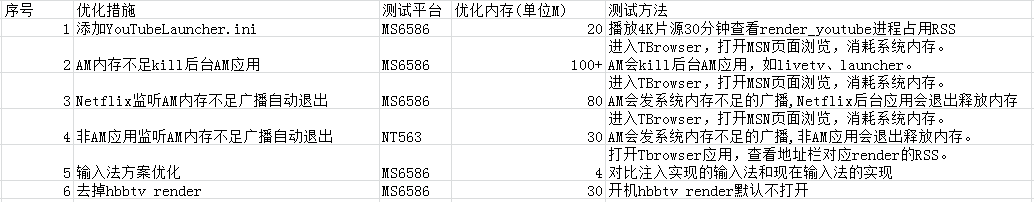
\includegraphics[width=\textwidth]{image/tbrw2_app_optimization/total.png} 
  \caption{优化措施总览}
\end{figure}

\newpage
%---------------------------------------------------------------------
\section{TBrowser2.0内存优化}
\subsection{优化方法}
\begin{figure}[H]
  \centering
  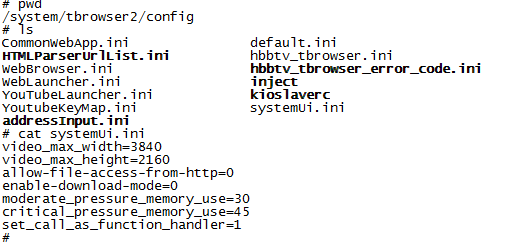
\includegraphics[width=10cm,height=5cm]{image/tbrw2_app_optimization/ini.png} 
  \caption{6586 配置文件}
\end{figure}
如图所示,每个render在tbrowser2/config目录下都应该有对应的page\_name.ini,render\_name与调用tos\_tbrowser接口所传的page\_name一样。在这个ini应该要包含moderate\_pressure\_memory\_use和critical\_pressure\_memory\_use两个配置项。\par
其中moderate\_pressure\_memory\_use代表render内存使用超过这个值浏览器将开始回收内存,critical\_pressure\_memory\_use代表render内存使用超过这个值浏览器将尽量多的回收内存。\par
这两个配置应该根据render的不同设置合理的值,比如render\_systemui内存使用在35M-50M之间,那么这个值应该设置为40M-45M。而render\_hbbtv内存使用普遍在120M-220M,那么这个值应该设置为160M-200M。
这样既可以限制render的峰值内存使用,同时又避免浏览器频繁回收内存造成用户体验不好。\par
优化效果:systemui添加收阈值30-45,原来没有设置render\_systemui峰值55M,添加阈值之后峰值41M。预计节约14M。
\subsection{实现原理}
\subsubsection{MemoryPressureListener}
\begin{figure}[H]
  \centering
  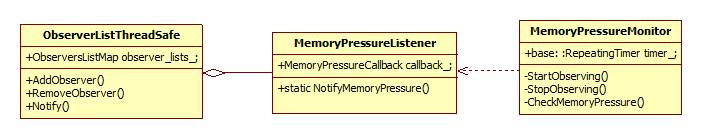
\includegraphics[width=\textwidth]{image/tbrw2_app_optimization/tbrw_memory_monitor.jpg}
  \caption{浏览器memory\_listener}
\end{figure}
1、浏览器内部模块如果需要进行内存回收,就在类中添加MemoryPressureListener成员变量,并设置OnMemoryPressure回调函数\par
2、MemoryPressureListener在构造函数调用g\_observers.Get().AddObserver(this);\par
3、MemoryPressureMonitor检测内存,通过MemoryPressureListener发送消息给所有MemoryPressureListener的子类\par

\subsubsection{MemoryPressureMonitor}
\begin{figure}[H]
  \centering
  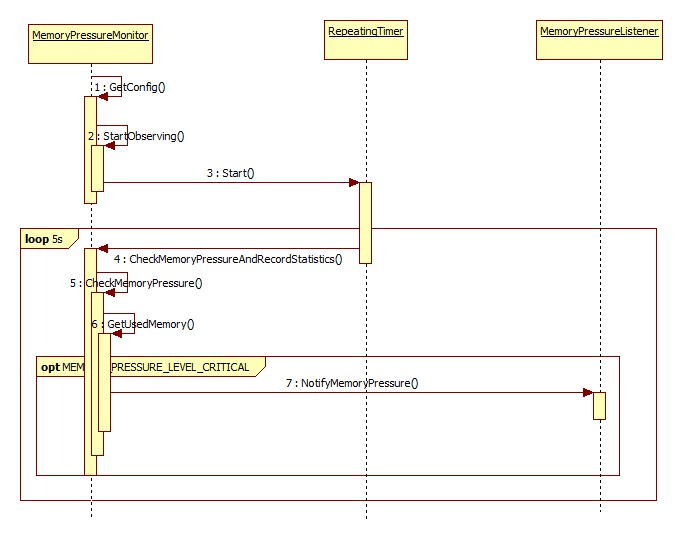
\includegraphics[width=\textwidth]{image/tbrw2_app_optimization/tbrw_memory_listener.jpg}
  \caption{浏览器memory\_monitor}
\end{figure}
1、getconfig获取ini文件里面配置的render回收的阈值moderate\_pressure\_memory\_use和critical\_pressure\_memory\_use\par
2、MemoryPressureMonitor初始化时启动一个timer,循环调用CheckMemoryPressureAndRecordStatistics用来判断内存使用情况\par
3、GetUsedMemory通过获取系统信息得到浏览器进程使用内存,通过与回收阈值对比得到是否应该进行内存回收\par
4、当内存使用超过moderate\_pressure\_memory\_use发送MEMORY\_PRESSURE\_LEVEL\_MODERATE给所有注册的listener,此时listenser回收可回收内存的一半\par
当内存使用超过critical\_pressure\_memory\_use发送MEMORY\_PRESSURE\_LEVEL\_CRITICAL给所有注册的listener,此时listenser回收可回收内存的一半

%---------------------------------------------------------------------

\section{AM应用内存优化}
\subsection{AM判断应用进程优先级}
\begin{table}[!htbp]   
\newcommand{\tabincell}[2]{\begin{tabular}{@{}#1@{}}#2\end{tabular}}   
  \begin{center}
  \caption{Android进程优先级}
  \label{table1}
  \begin{tabular}{|l|l|}      
  \hline                     
  优先级 & 简介\\
  \hline        
  IMPORTANCE\_FOREGROUND & 前台进程:它表明用户正在与该进程进行交互操作。 \\  \hline 
  IMPORTANCE\_VISIBLE & \tabincell{l}{可见进程:它表明虽然该进程没有持有任何前台组件,\\但是它还是能够影响到用户看得到的界面。} \\  \hline 
  IMPORTANCE\_SERVICE & \tabincell{l}{服务进程:除了符合前台进程和可见进程条件的Service,\\其它的Service都会被归类为服务进程。} \\ \hline
  IMPORTANCE\_BACKGROUND & \tabincell{l}{后台进程:持有不可见Activity(调用了onStop()方法)\\的进程即为后台进程。} \\ \hline
  IMPORTANCE\_EMPTY & 空进程:不持有任何活动组件的进程。 \\
  \hline
  \end{tabular}
  \end{center}
  \end{table}
参考以上Android进程优先级,我们结合自身应用特点,设置如下进程优先级,优先级从高到低:
\begin{table}[!htbp]      
  \begin{center}
  \caption{AM进程优先级}
  \label{table2}
  \begin{tabular}{|l|l|}
  \hline                     
  优先级 & 简介\\
  \hline        
  IMPORTANCE\_HOME\_APP & 根应用进程:system\_ui应用。 \\ \hline
  IMPORTANCE\_UNABLE\_TO\_KILL & 不可被kill进程:例如cross\_ui应用。 \\ \hline
  IMPORTANCE\_FOREGROUND & 前台进程:它表明用户正在与该进程进行交互操作。 \\  \hline 
  IMPORTANCE\_PERSISTED & 重要服务进程:persisted为true的服务进程。 \\ \hline
  IMPORTANCE\_BACKGROUND & 后台进程:后台应用进程和后台服务进程。\\
  \hline
  \end{tabular}
  \end{center}
  \end{table}
\begin{enumerate}
  \item 第一组:优先级为IMPORTANCE\_BACKGROUND的后台进程,主要指服务进程。我们将这些组件存储在run\_apps\_list中。
  \item 第二组:优先级为IMPORTANCE\_PERSISTED的服务进程,我们将第二组服务存储在persistent\_ser\_list中。
  \item 第三组:优先级为IMPORTANCE\_FOREGROUND的应用进程及bind的service。
\end{enumerate}
\subsection{AM循环检测系统内存}
\begin{figure}[H] 
  \centering 
  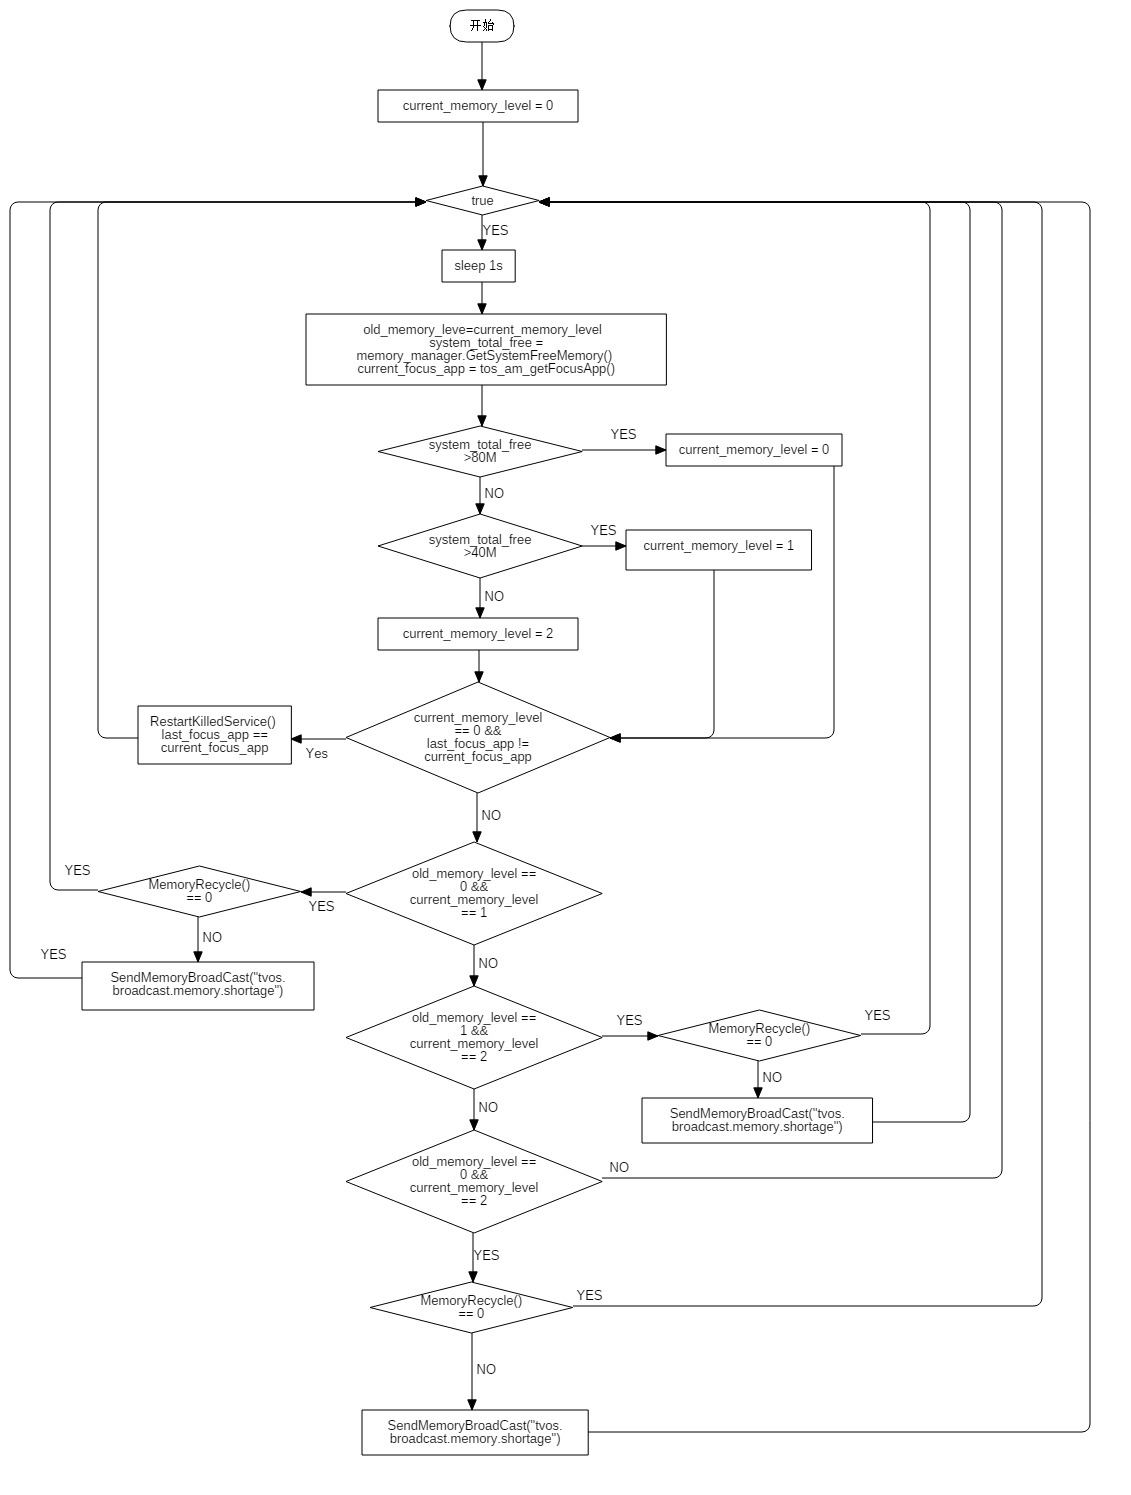
\includegraphics[width=17cm,height=21cm]{image/tbrw2_app_optimization/png/memory_check.jpg}
  \caption{AM循环检测系统内存}
\end{figure}
AM启动参数中设置recycle\_size = 80M和recycle\_critical\_size = 40M,不同平台可以设置不同的值\par
\begin{itemize}
  \item 系统free memory 大于recycle\_size,依据系统剩余内存大小,设置内存状态等级为0,可以尝试启动不是在当前应用活动状态下退出的应用进程。
  \item 系统free memory 大于recycle\_critical\_size,小于recycle\_size,设置内存状态等级为1。
  \item 系统free memory 小于recycle\_critical\_size,设置内存等级为2。
\end{itemize}
\begin{table}[!htbp]
  \begin{center}
  \caption{剩余内存大小与内存状态对应表}
  \label{biao}
  \begin{tabular}{|l|l|}      
  \hline                     
  剩余内存大小 & 系统内存状态\\
  \hline        
  free memory > 80M & AM\_MEMORY\_PRESSURE\_LEVEL\_NONE (0) \\  \hline 
  40M < free memory < 80M & AM\_MEMORY\_PRESSURE\_LEVEL\_MODERATE (1) \\  \hline 
  free memory < 40M & AM\_MEMORY\_PRESSURE\_LEVEL\_CRITICAL (2) \\
  \hline
  \end{tabular}
  \end{center}
  \end{table}
\par 当状态由0变为1时,由1变为2,由0变为2时,运行MemoryRecycle()回收内存,若成功则返回继续监测内存,若未成功,则发送“tvos.broadcast.memory.shortage”广播,传递系统剩余内存大小及当前系统内存状态变化信息。
其中date中传递剩余内存大小数据,extra\_data中传递系统状态变化信息。
\subsection{AM kill后台应用时序图}
\begin{figure}[H]
  \centering
  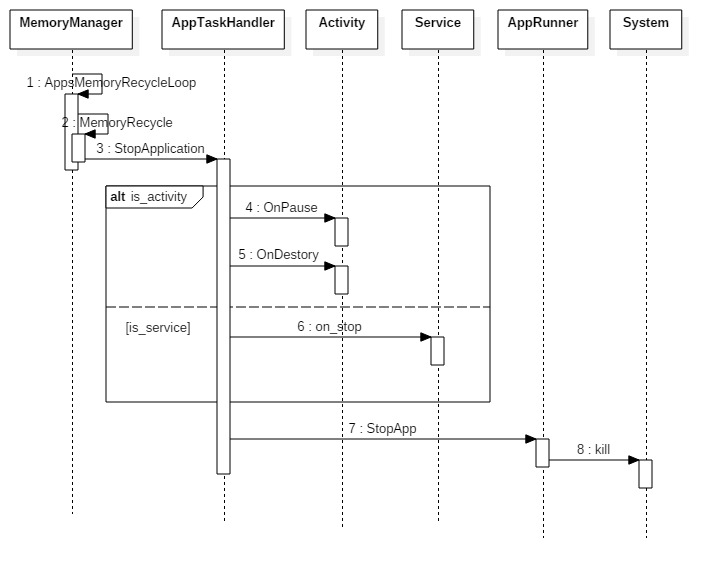
\includegraphics[width=\textwidth]{image/tbrw2_app_optimization/png/kill_progress.jpg}
  \caption{AM kill后台应用时序图}
\end{figure}
依据系统内存状态,选择退出不同优先级的activity或者service。\par
当状态由0变为1时,kill掉第一组进程。\par
当状态由1变为2时,kill掉第二组进程。若此后状态仍然为2,那么为了保证系统稳定,需要将当前的前台进程,即第三组进程kill掉。\par
当状态由0变为2时,先kill掉第一组应用,若内存状态变为了1,那么就暂时不做处理,若状态仍持续为2,则kill掉persisted设置为true的service。\par
%---------------------------------------------------------------------

\section{非AM应用管理与内存优化}
\subsection{非AM应用管理}
非AM应用由一个开机启动的service管理,这个service优先级为IMPORTANCE\_PERSISTED,管理若干非AM应用,无法退出的非AM应用无法被该service管理。

\subsection{NotAMApp开机启动流程}
\begin{figure}[H]
  \centering
  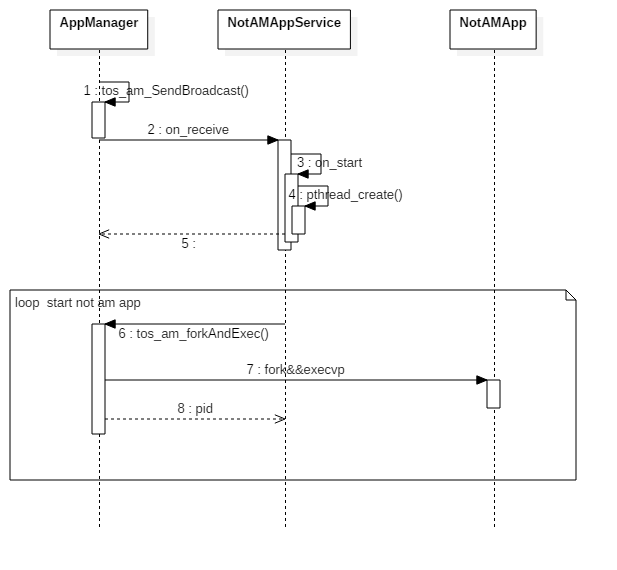
\includegraphics[width=\textwidth]{image/tbrw2_app_optimization/png/start_not_am_app.png}
  \caption{NotAMApp开机启动时序图}
\end{figure}
NotAMApp服务启动后创建一个线程去启动管理的应用,避免拖慢开机速度。根据各平台的应用开启现状,在开启应用时需要sleep若干时间,避免占用CPU导致开机速度变慢。

\subsection{NotAMApp退出重启流程}
\begin{figure}[H]
  \centering
  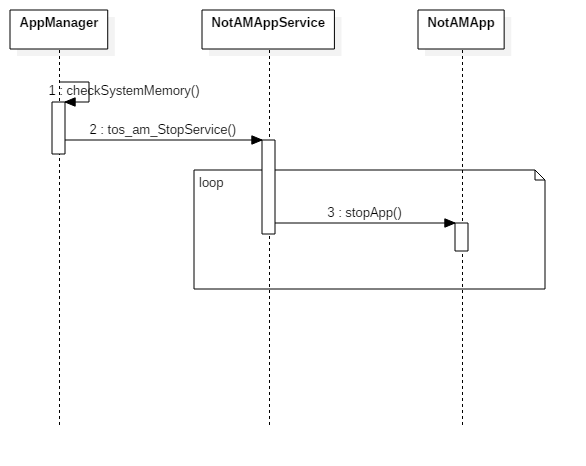
\includegraphics[width=\textwidth]{image/tbrw2_app_optimization/png/stop_not_am_app.png}
  \caption{NotAMApp退出重启时序图}
\end{figure}
NotAMApp退出时,会将管理的所有非AM应用关闭。
%1、收到AM广播TOS\_AM\_MEMORY\_PRESSURE\_LEVEL\_MODERATE退出优先级低的应用,发TOS\_AM\_MEMORY\_PRESSURE\_LEVEL\_CRITICAL退出所有管理的应用。应用退出时记录当前focus\_app\par
%2、收到AM广播TOS\_AM\_MEMORY\_PRESSURE\_LEVEL\_NONE准备重启已退出的应用,需要对比当前focus\_app与退出时记录的focus\_app,如果不一样才重启。这样可以避免频繁退出重启。

%---------------------------------------------------------------------

\section{tbrw2应用优化}
\subsection{输入法方案优化}
原输入法是以注入的形式注入到页面中使用,并且在每一个用到输入法的应用中均需要包含对输入法处理的代码,会造成代码冗余。新输入法代码只包含一份,便于管理,并且可以节约4M左右的内存。\par
新输入法只适用于基于 TbrowserActivity 类开发的应用。\par
\subsection{Netflix监听AM内存广播}
Netflix常驻后台会占用80M左右内存,通过监听tvos.broadcast.memory.shortage广播,在内存使用级别为1时主动退出,能释放80M的内存。
\subsection{提供设置ipad useragent的页面}
TBrowser应用提供了设置UA的选择框,可以选择pc UA或者ipad UA。使用ipad UA访问某些页面可以节约内存。
\subsection{巧用TbrowserActivity基类}
TbrowserActivity基类实现了中间件消息回调函数、浏览器消息回调函数、输入法等基础功能,子类如果使用了这些方法能少写很多代码。
\subsection{hbbtv render优化}
原来hbbtv开机启动会调用tos\_tbrowser\_load\_url\_with\_name(PAGE\_NAME, about:blank);导致后台一直有hbbtv的render进程。\par
现在代码已经去掉这句话,等真正有需要打开hbbtv页面的时候直接打开正确的页面,这样可以节约30M左右内存。
%---------------------------------------------------------------------

\ifx\withtbrowser\undefined
\else
\section{Extension Framework使用到的v8 API}

FunctionTemplate类是Function类的模板类,可以理解为设置Function的公共特性,
通过FunctionTemplate类new出来的Function类就拥有这些特性。相当于页面的function。
\begin{spacing}{1.0}
\begin{lstlisting}[language={C++}]
/**
@brief new一个FunctionTemplate对象

@param[in] isolate表示一个独立的v8引擎实例,每个实例维护不同的状态
@param[in] callback是回调函数,创建实例或方法被调用时会调用
@param[in] data表示给回调函数传递的额外的参数
@return 返回FunctionTemplate对象
*/
static Local<FunctionTemplate> New(
    Isolate* isolate, FunctionCallback callback = 0,
    Local<Value> data = Local<Value>(),
    Local<Signature> signature = Local<Signature>(), int length = 0,
    ConstructorBehavior behavior = ConstructorBehavior::kAllow);

/**
 * Set the call-handler callback for a FunctionTemplate.  This
 * callback is called whenever the function created from this
 * FunctionTemplate is called.
 */
void SetCallHandler(FunctionCallback callback,
    Local<Value> data = Local<Value>());
\end{lstlisting}
\end{spacing}

ObjectTemplate类是Object类的模板类,可以理解为设置Object的公共特性,
通过ObjectTemplate类new出来的Object类就拥有这些特性。相当于页面的object。
\begin{spacing}{1.0}
\begin{lstlisting}[language={C++}]
/**
@brief new一个ObjectTemplate对象

@param[in] isolate表示一个独立的v8引擎实例,每个实例维护不同的状态
@param[in] constructor是默认构造函数,只用于创建实例时会调用
@return 返回ObjectTemplate对象
*/
static Local<ObjectTemplate> New(
    Isolate* isolate,
    Local<FunctionTemplate> constructor = Local<FunctionTemplate>());

/**
@brief new一个Object对象实例

@param[in] context表示JavaScript代码运行环境上下文
@return 返回Object对象
*/
V8_WARN_UNUSED_RESULT MaybeLocal<Object> NewInstance(Local<Context> context);

/**
@brief 能够指定JavaScript访问对象属性时的一个callback

@param[in] getter表示获取属性时会被调用的callback
@param[in] setter表示设置属性时会被调用的callback
*/
void SetNamedPropertyHandler(NamedPropertyGetterCallback getter,
    NamedPropertySetterCallback setter = 0,
    NamedPropertyQueryCallback query = 0,
    NamedPropertyDeleterCallback deleter = 0,
    NamedPropertyEnumeratorCallback enumerator = 0,
    Local<Value> data = Local<Value>());
    
/**
@brief 通过这个模板生成的Object对象可以设置的内部field的数量

@param[in] value表示设置内部field的数量
*/
void SetInternalFieldCount(int value);
\end{lstlisting}
\end{spacing}

Object类是一个实例对象
\begin{spacing}{1.0}
\begin{lstlisting}[language={C++}]
/**
@brief 设置Object的内部field

@param[in] index表示Object的内部field的索引值,必须小于SetInternalFieldCount函数传入的值
@param[in] value表示Object的内部field值
*/
void SetInternalField(int index, Local<Value> value);
\end{lstlisting}
\end{spacing}

其他
\begin{spacing}{1.0}
\begin{lstlisting}[language={C++}]
/**
 * A map that uses Global as value and std::map as the backing
 * implementation. Globals are held non-weak.
 *
 * C++11 embedders don't need this class, as they can use
 * Global directly in std containers.
 */
template <typename K, typename V,
          typename Traits = DefaultGlobalMapTraits<K, V> >
class StdGlobalValueMap : public GlobalValueMap<K, V, Traits> {
 public:
  explicit StdGlobalValueMap(Isolate* isolate)
      : GlobalValueMap<K, V, Traits>(isolate) {}
};
\end{lstlisting}
\end{spacing}

\section{extension framework架构分析}
\begin{figure}[H] 
  \centering 
  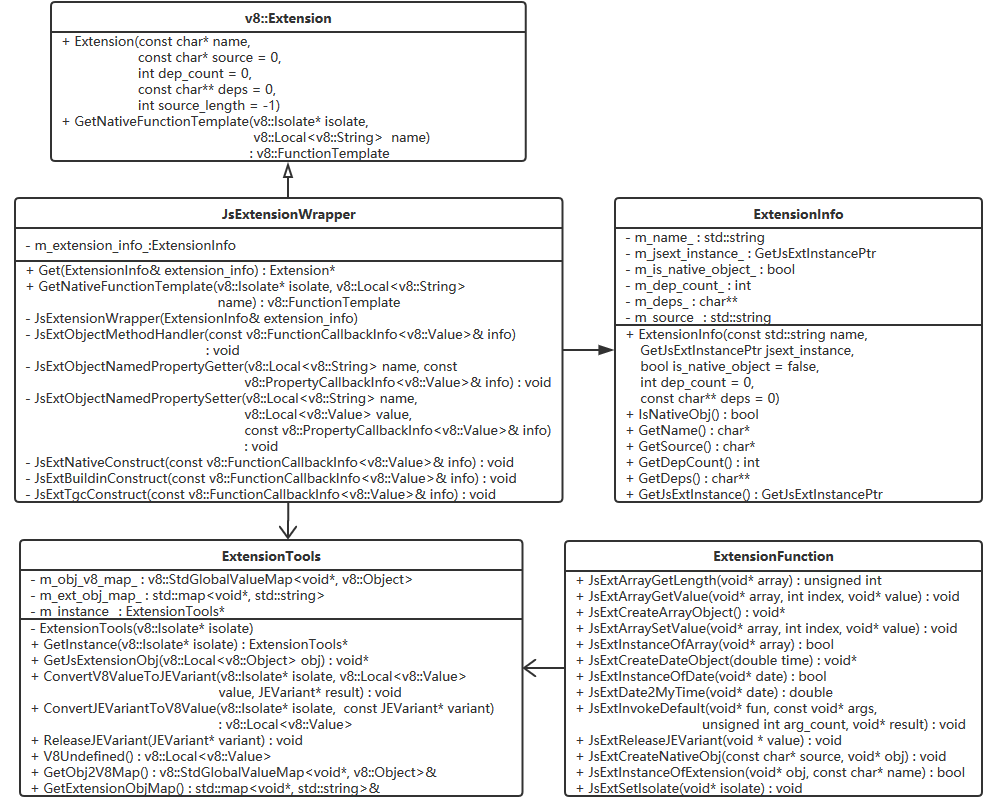
\includegraphics[width=\textwidth]{image/extension_framework/extension_framework_class.png} 
  \caption{extension framwork静态类图} \label{fig:extension_framework_class} 
\end{figure}

如第图~\ref{fig:extension_framework_class}所示:
v8扩展机制主要是继承v8内置的Extension类,通过重写其GetNativeFunctionTemplate方法来获取FunctionTemplate对象;
JsExtensionWrapper类主要就是封装创建出来的FunctionTemplate对象的一些特性,比如构造函数,属性拦截器,方法执行;
ExtensionInfo类主要记录了创建v8扩展所有需要的关键信息;ExtensionTools类主要是提供简易的函数,比如通过v8::Object类获取ExtensionBase对象,
将v8变量转换为扩展变量,将扩展变量转换为v8变量,释放扩展变量等;ExtensionFunction主要提供常用对外接口给js扩展调用。

\begin{figure}[H] 
  \centering 
  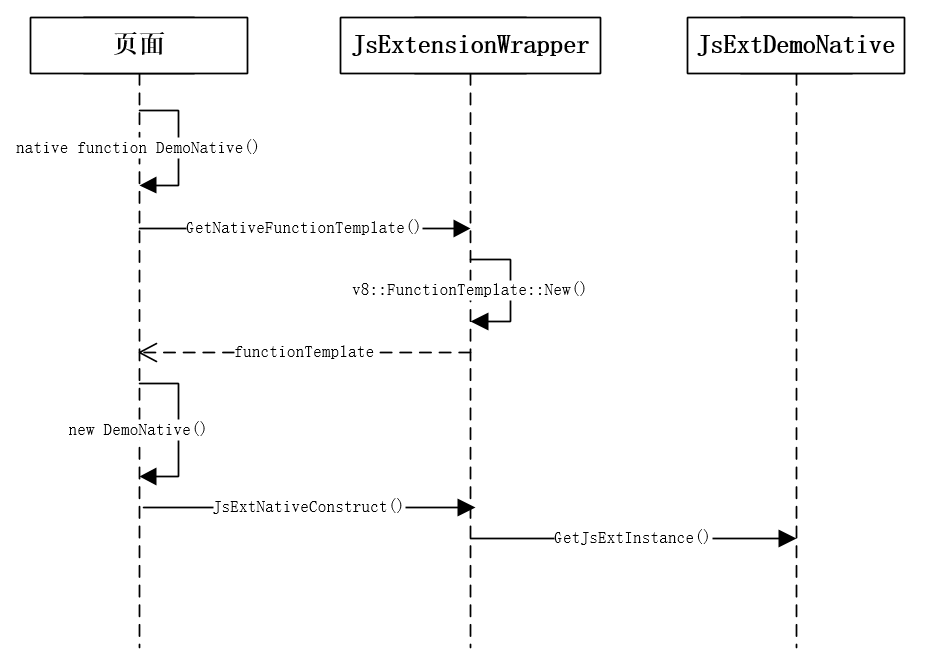
\includegraphics[width=\textwidth]{image/extension_framework/extension_construct_sequence.png} 
  \caption{js扩展对象创建时序图} \label{fig:extension_construct_sequence} 
\end{figure}

js扩展对象创建时序图如图~\ref{fig:extension_construct_sequence}所示:
\begin{itemize}
  \item 在页面加载时,v8::extension会注入页面代码native function DemoNative(),此时v8就会去创建DemoNative对应functionTemplate模板类。
  \item 当web开发人员在页面使用new DemoNative()时,functionTemplate模板类就会返回一个v8::Object实例对象给页面。
  \item 同理,针对内置对象,v8::extension会注入页面代码native function DemoBuildin()和var DemoBuildin = DemoBuildin()两段代码,
  此时由于DemoBuildin变量覆盖了DemoBuildin方法名,所以只能通过DemoBuildin执行对应方法和函数,不能再被new。
\end{itemize}

\begin{figure}[H] 
  \centering 
  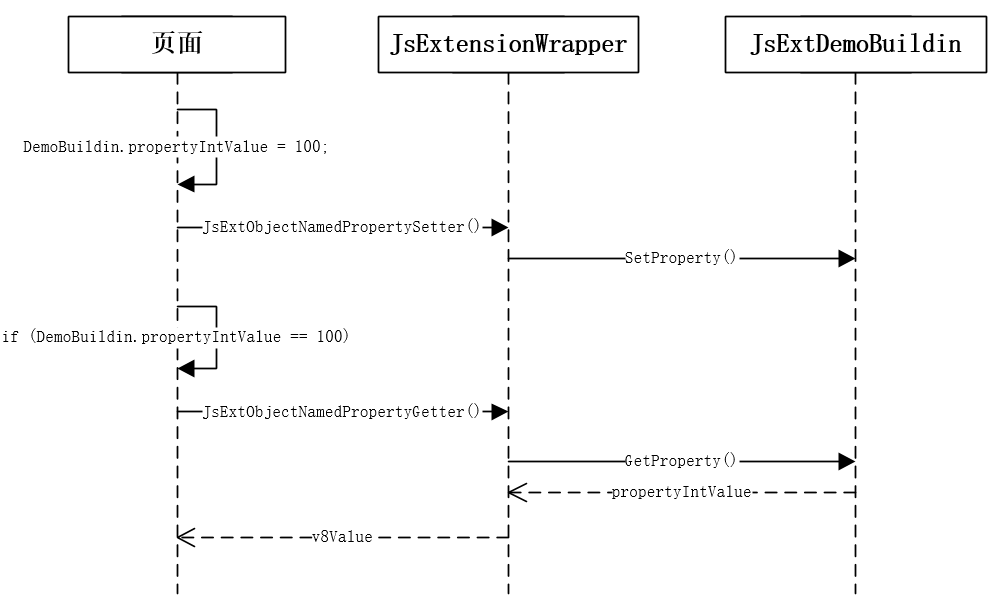
\includegraphics[width=\textwidth]{image/extension_framework/extension_property_sequence.png} 
  \caption{js扩展对象属性访问时序图} \label{fig:extension_property_sequence} 
\end{figure}

js扩展对象属性访问时序图如图~\ref{fig:extension_property_sequence}所示:
\begin{itemize}
  \item 由于在创建DemoBuildin对象时,对其ObjectTemplate模板类设置了拦截器特性,所以任何属性访问都会调用到拦截器的回调方法里。
\end{itemize}

\begin{figure}[H] 
  \centering 
  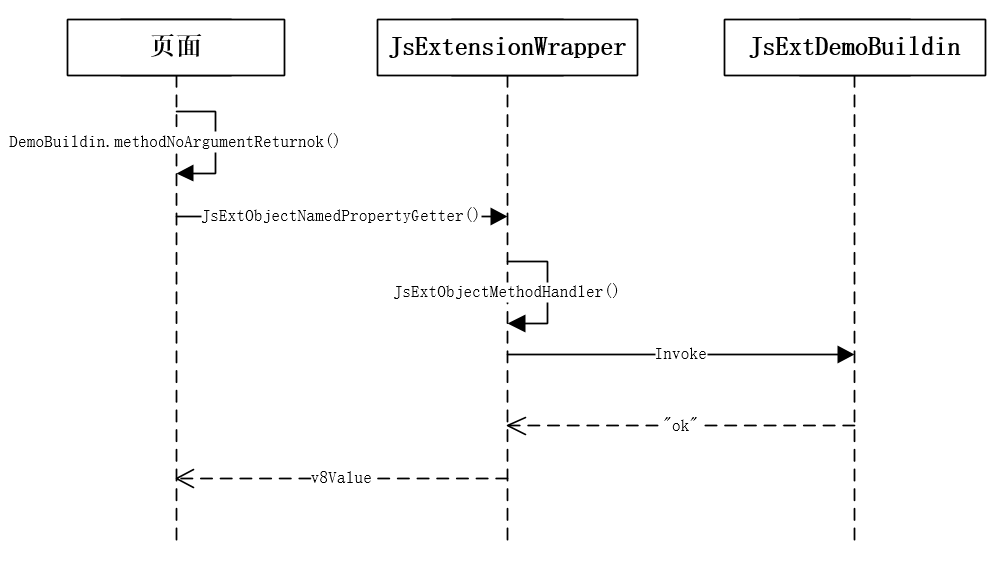
\includegraphics[width=\textwidth]{image/extension_framework/extension_function_sequence.png} 
  \caption{js扩展对象方法访问时序图} \label{fig:extension_function_sequence} 
\end{figure}

js扩展对象方法访问时序图如图~\ref{fig:extension_function_sequence}所示:
\begin{itemize}
  \item 同获取属性流程一致,当在拦截器回调函数里查询,如果属性没找到调用名,就去方法里找。
\end{itemize}

\section{Extension Framework垃圾回收机制}

对于内置对象,每次跳转页面,都会去调用其构造函数,此时回收机制的做法是先delete上个页面new出来的js扩展实例对象,再重新new一个js扩展实例对象,
然后绑定到v8 Object对象里。
\begin{spacing}{1.0}
\begin{lstlisting}[language={C++}]
void* delete_obj = ExtensionTools::GetJsExtensionObj(v8_obj);
  if (delete_obj) {
    ExtensionBase* ext_base = static_cast<ExtensionBase*>(delete_obj);
    delete ext_base;
    ext_base = NULL;
  }

  void* new_obj = NULL;
  extension_info->GetJsExtInstance()(NULL, 0, &new_obj);
  v8_obj->SetInternalField(ExtensionTools::JsExtBaseInternalField, v8::External::New(isolate, new_obj));
\end{lstlisting}
\end{spacing}

对于本地对象,每次创建对象时,我们会通过一个std::map保存js扩展实例对象指针以及name,当跳转页面,都会去调用tgc内置对象其构造函数,
将这个map里js扩展实例对象指针全部delete掉。
\begin{spacing}{1.0}
\begin{lstlisting}[language={C++}]
//在构造函数中将js扩展实例对象指针以及name保存到一个map中
void JsExtensionWrapper::JsExtNativeConstruct(const FunctionCallbackInfo<v8::Value>& info) {
  ...
  ExtensionTools* extension_tools = ExtensionTools::GetInstance(isolate);
  extension_tools->GetExtensionObjMap().insert(std::pair<void*, std::string>(new_obj, extension_info->GetName()));
  ...
}

//在tgc内置对象构造函数中将map中的js扩展实例对象指针全部delete掉
void JsExtensionWrapper::JsExtTgcConstruct(const FunctionCallbackInfo<v8::Value>& info) {
  ...
  ExtensionTools* extension_tools = ExtensionTools::GetInstance(isolate);
  std::map<void*, std::string>::iterator it;
  for (it = extension_tools->GetExtensionObjMap().begin(); it != extension_tools->GetExtensionObjMap().end(); it++) {
    ExtensionBase* ext_base = static_cast<ExtensionBase*>(it->first);
    if (ext_base) {
      delete ext_base;
      ext_base = NULL;
    }
  }
  ...
}
\end{lstlisting}
\end{spacing}



%---------------------------------------------------------------------

\ifx\withtbrowser\undefined
\else
\section{Extension Framework使用到的v8 API}

FunctionTemplate类是Function类的模板类,可以理解为设置Function的公共特性,
通过FunctionTemplate类new出来的Function类就拥有这些特性。相当于页面的function。
\begin{spacing}{1.0}
\begin{lstlisting}[language={C++}]
/**
@brief new一个FunctionTemplate对象

@param[in] isolate表示一个独立的v8引擎实例,每个实例维护不同的状态
@param[in] callback是回调函数,创建实例或方法被调用时会调用
@param[in] data表示给回调函数传递的额外的参数
@return 返回FunctionTemplate对象
*/
static Local<FunctionTemplate> New(
    Isolate* isolate, FunctionCallback callback = 0,
    Local<Value> data = Local<Value>(),
    Local<Signature> signature = Local<Signature>(), int length = 0,
    ConstructorBehavior behavior = ConstructorBehavior::kAllow);

/**
 * Set the call-handler callback for a FunctionTemplate.  This
 * callback is called whenever the function created from this
 * FunctionTemplate is called.
 */
void SetCallHandler(FunctionCallback callback,
    Local<Value> data = Local<Value>());
\end{lstlisting}
\end{spacing}

ObjectTemplate类是Object类的模板类,可以理解为设置Object的公共特性,
通过ObjectTemplate类new出来的Object类就拥有这些特性。相当于页面的object。
\begin{spacing}{1.0}
\begin{lstlisting}[language={C++}]
/**
@brief new一个ObjectTemplate对象

@param[in] isolate表示一个独立的v8引擎实例,每个实例维护不同的状态
@param[in] constructor是默认构造函数,只用于创建实例时会调用
@return 返回ObjectTemplate对象
*/
static Local<ObjectTemplate> New(
    Isolate* isolate,
    Local<FunctionTemplate> constructor = Local<FunctionTemplate>());

/**
@brief new一个Object对象实例

@param[in] context表示JavaScript代码运行环境上下文
@return 返回Object对象
*/
V8_WARN_UNUSED_RESULT MaybeLocal<Object> NewInstance(Local<Context> context);

/**
@brief 能够指定JavaScript访问对象属性时的一个callback

@param[in] getter表示获取属性时会被调用的callback
@param[in] setter表示设置属性时会被调用的callback
*/
void SetNamedPropertyHandler(NamedPropertyGetterCallback getter,
    NamedPropertySetterCallback setter = 0,
    NamedPropertyQueryCallback query = 0,
    NamedPropertyDeleterCallback deleter = 0,
    NamedPropertyEnumeratorCallback enumerator = 0,
    Local<Value> data = Local<Value>());
    
/**
@brief 通过这个模板生成的Object对象可以设置的内部field的数量

@param[in] value表示设置内部field的数量
*/
void SetInternalFieldCount(int value);
\end{lstlisting}
\end{spacing}

Object类是一个实例对象
\begin{spacing}{1.0}
\begin{lstlisting}[language={C++}]
/**
@brief 设置Object的内部field

@param[in] index表示Object的内部field的索引值,必须小于SetInternalFieldCount函数传入的值
@param[in] value表示Object的内部field值
*/
void SetInternalField(int index, Local<Value> value);
\end{lstlisting}
\end{spacing}

其他
\begin{spacing}{1.0}
\begin{lstlisting}[language={C++}]
/**
 * A map that uses Global as value and std::map as the backing
 * implementation. Globals are held non-weak.
 *
 * C++11 embedders don't need this class, as they can use
 * Global directly in std containers.
 */
template <typename K, typename V,
          typename Traits = DefaultGlobalMapTraits<K, V> >
class StdGlobalValueMap : public GlobalValueMap<K, V, Traits> {
 public:
  explicit StdGlobalValueMap(Isolate* isolate)
      : GlobalValueMap<K, V, Traits>(isolate) {}
};
\end{lstlisting}
\end{spacing}

\section{extension framework架构分析}
\begin{figure}[H] 
  \centering 
  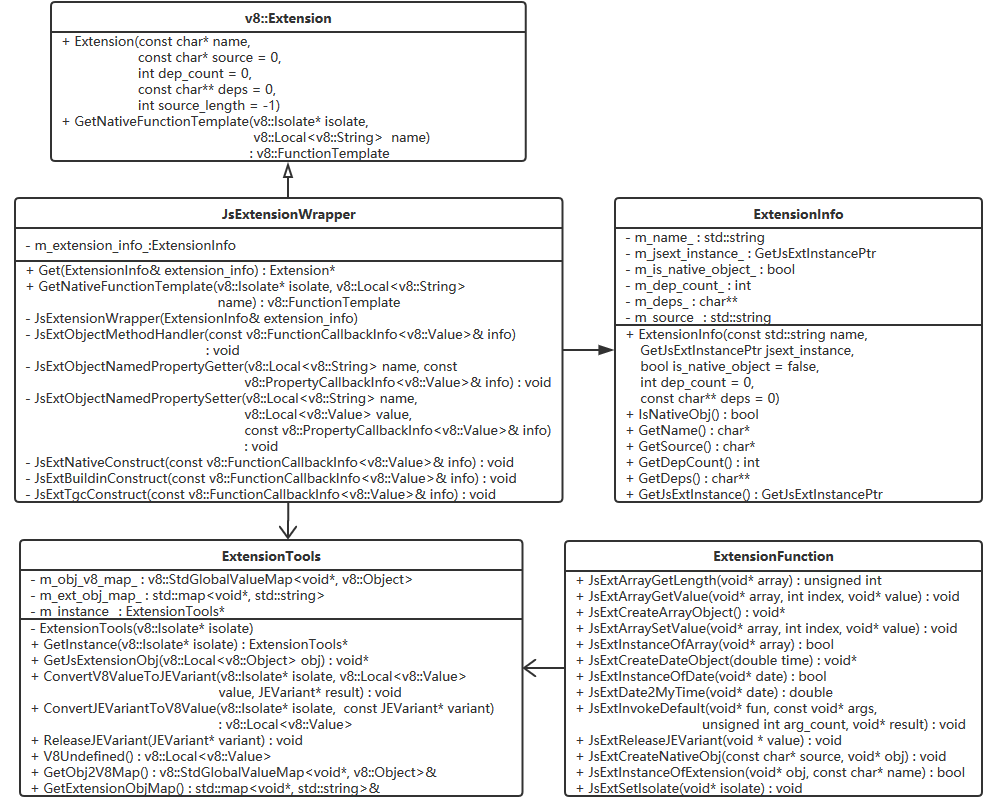
\includegraphics[width=\textwidth]{image/extension_framework/extension_framework_class.png} 
  \caption{extension framwork静态类图} \label{fig:extension_framework_class} 
\end{figure}

如第图~\ref{fig:extension_framework_class}所示:
v8扩展机制主要是继承v8内置的Extension类,通过重写其GetNativeFunctionTemplate方法来获取FunctionTemplate对象;
JsExtensionWrapper类主要就是封装创建出来的FunctionTemplate对象的一些特性,比如构造函数,属性拦截器,方法执行;
ExtensionInfo类主要记录了创建v8扩展所有需要的关键信息;ExtensionTools类主要是提供简易的函数,比如通过v8::Object类获取ExtensionBase对象,
将v8变量转换为扩展变量,将扩展变量转换为v8变量,释放扩展变量等;ExtensionFunction主要提供常用对外接口给js扩展调用。

\begin{figure}[H] 
  \centering 
  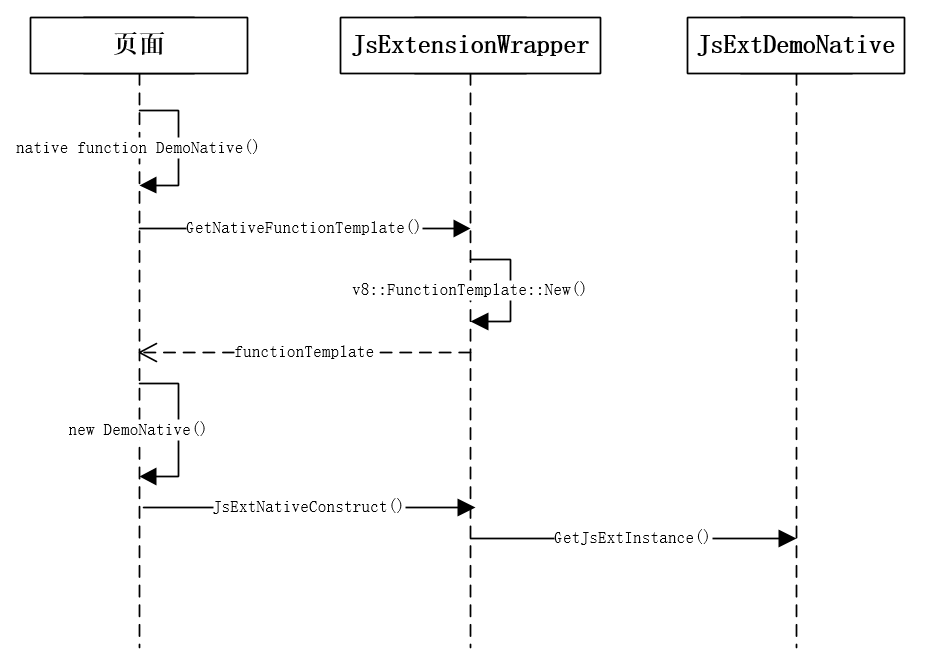
\includegraphics[width=\textwidth]{image/extension_framework/extension_construct_sequence.png} 
  \caption{js扩展对象创建时序图} \label{fig:extension_construct_sequence} 
\end{figure}

js扩展对象创建时序图如图~\ref{fig:extension_construct_sequence}所示:
\begin{itemize}
  \item 在页面加载时,v8::extension会注入页面代码native function DemoNative(),此时v8就会去创建DemoNative对应functionTemplate模板类。
  \item 当web开发人员在页面使用new DemoNative()时,functionTemplate模板类就会返回一个v8::Object实例对象给页面。
  \item 同理,针对内置对象,v8::extension会注入页面代码native function DemoBuildin()和var DemoBuildin = DemoBuildin()两段代码,
  此时由于DemoBuildin变量覆盖了DemoBuildin方法名,所以只能通过DemoBuildin执行对应方法和函数,不能再被new。
\end{itemize}

\begin{figure}[H] 
  \centering 
  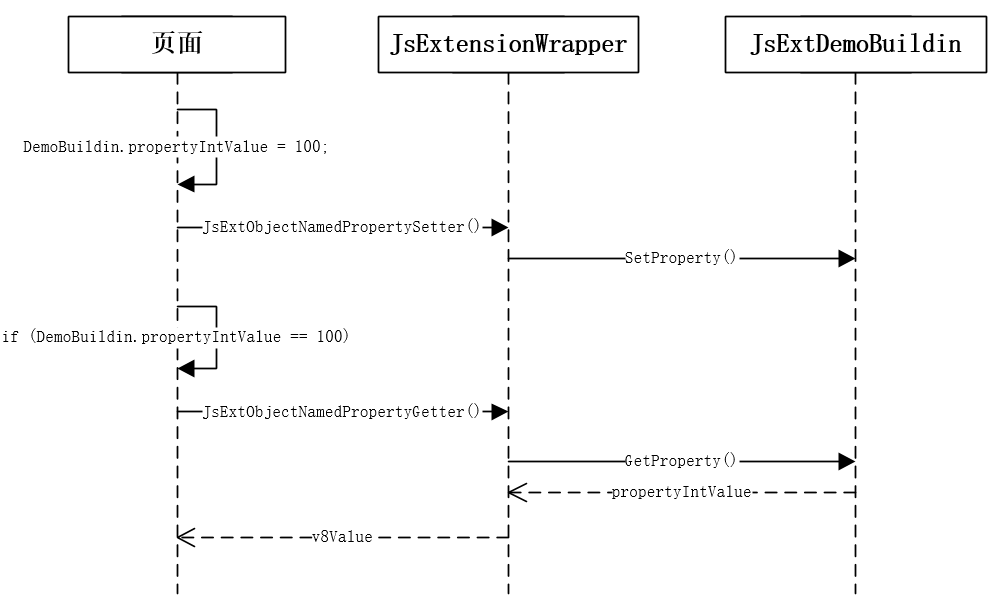
\includegraphics[width=\textwidth]{image/extension_framework/extension_property_sequence.png} 
  \caption{js扩展对象属性访问时序图} \label{fig:extension_property_sequence} 
\end{figure}

js扩展对象属性访问时序图如图~\ref{fig:extension_property_sequence}所示:
\begin{itemize}
  \item 由于在创建DemoBuildin对象时,对其ObjectTemplate模板类设置了拦截器特性,所以任何属性访问都会调用到拦截器的回调方法里。
\end{itemize}

\begin{figure}[H] 
  \centering 
  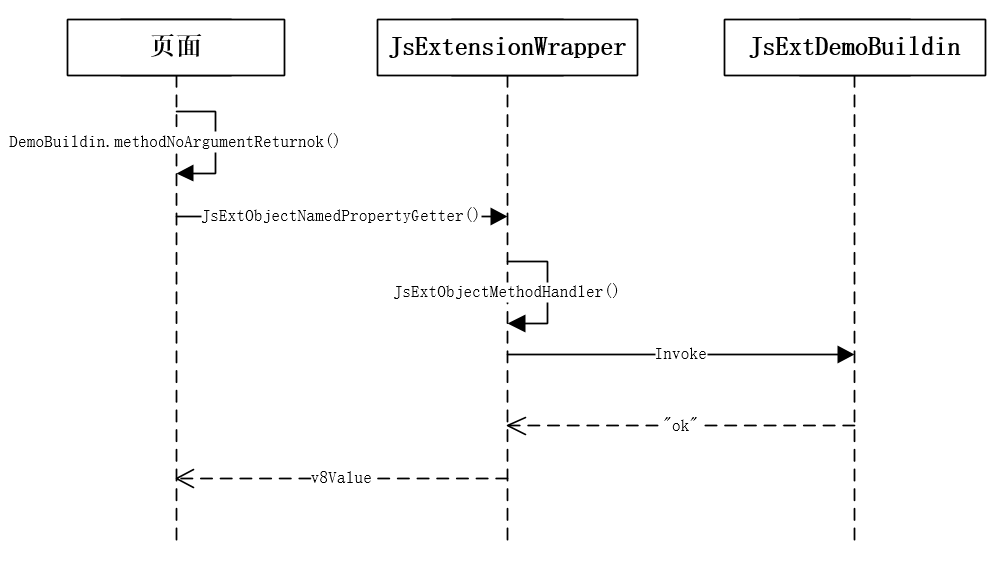
\includegraphics[width=\textwidth]{image/extension_framework/extension_function_sequence.png} 
  \caption{js扩展对象方法访问时序图} \label{fig:extension_function_sequence} 
\end{figure}

js扩展对象方法访问时序图如图~\ref{fig:extension_function_sequence}所示:
\begin{itemize}
  \item 同获取属性流程一致,当在拦截器回调函数里查询,如果属性没找到调用名,就去方法里找。
\end{itemize}

\section{Extension Framework垃圾回收机制}

对于内置对象,每次跳转页面,都会去调用其构造函数,此时回收机制的做法是先delete上个页面new出来的js扩展实例对象,再重新new一个js扩展实例对象,
然后绑定到v8 Object对象里。
\begin{spacing}{1.0}
\begin{lstlisting}[language={C++}]
void* delete_obj = ExtensionTools::GetJsExtensionObj(v8_obj);
  if (delete_obj) {
    ExtensionBase* ext_base = static_cast<ExtensionBase*>(delete_obj);
    delete ext_base;
    ext_base = NULL;
  }

  void* new_obj = NULL;
  extension_info->GetJsExtInstance()(NULL, 0, &new_obj);
  v8_obj->SetInternalField(ExtensionTools::JsExtBaseInternalField, v8::External::New(isolate, new_obj));
\end{lstlisting}
\end{spacing}

对于本地对象,每次创建对象时,我们会通过一个std::map保存js扩展实例对象指针以及name,当跳转页面,都会去调用tgc内置对象其构造函数,
将这个map里js扩展实例对象指针全部delete掉。
\begin{spacing}{1.0}
\begin{lstlisting}[language={C++}]
//在构造函数中将js扩展实例对象指针以及name保存到一个map中
void JsExtensionWrapper::JsExtNativeConstruct(const FunctionCallbackInfo<v8::Value>& info) {
  ...
  ExtensionTools* extension_tools = ExtensionTools::GetInstance(isolate);
  extension_tools->GetExtensionObjMap().insert(std::pair<void*, std::string>(new_obj, extension_info->GetName()));
  ...
}

//在tgc内置对象构造函数中将map中的js扩展实例对象指针全部delete掉
void JsExtensionWrapper::JsExtTgcConstruct(const FunctionCallbackInfo<v8::Value>& info) {
  ...
  ExtensionTools* extension_tools = ExtensionTools::GetInstance(isolate);
  std::map<void*, std::string>::iterator it;
  for (it = extension_tools->GetExtensionObjMap().begin(); it != extension_tools->GetExtensionObjMap().end(); it++) {
    ExtensionBase* ext_base = static_cast<ExtensionBase*>(it->first);
    if (ext_base) {
      delete ext_base;
      ext_base = NULL;
    }
  }
  ...
}
\end{lstlisting}
\end{spacing}



%---------------------------------------------------------------------

\ifx\withtbrowser\undefined
\else
\section{Extension Framework使用到的v8 API}

FunctionTemplate类是Function类的模板类,可以理解为设置Function的公共特性,
通过FunctionTemplate类new出来的Function类就拥有这些特性。相当于页面的function。
\begin{spacing}{1.0}
\begin{lstlisting}[language={C++}]
/**
@brief new一个FunctionTemplate对象

@param[in] isolate表示一个独立的v8引擎实例,每个实例维护不同的状态
@param[in] callback是回调函数,创建实例或方法被调用时会调用
@param[in] data表示给回调函数传递的额外的参数
@return 返回FunctionTemplate对象
*/
static Local<FunctionTemplate> New(
    Isolate* isolate, FunctionCallback callback = 0,
    Local<Value> data = Local<Value>(),
    Local<Signature> signature = Local<Signature>(), int length = 0,
    ConstructorBehavior behavior = ConstructorBehavior::kAllow);

/**
 * Set the call-handler callback for a FunctionTemplate.  This
 * callback is called whenever the function created from this
 * FunctionTemplate is called.
 */
void SetCallHandler(FunctionCallback callback,
    Local<Value> data = Local<Value>());
\end{lstlisting}
\end{spacing}

ObjectTemplate类是Object类的模板类,可以理解为设置Object的公共特性,
通过ObjectTemplate类new出来的Object类就拥有这些特性。相当于页面的object。
\begin{spacing}{1.0}
\begin{lstlisting}[language={C++}]
/**
@brief new一个ObjectTemplate对象

@param[in] isolate表示一个独立的v8引擎实例,每个实例维护不同的状态
@param[in] constructor是默认构造函数,只用于创建实例时会调用
@return 返回ObjectTemplate对象
*/
static Local<ObjectTemplate> New(
    Isolate* isolate,
    Local<FunctionTemplate> constructor = Local<FunctionTemplate>());

/**
@brief new一个Object对象实例

@param[in] context表示JavaScript代码运行环境上下文
@return 返回Object对象
*/
V8_WARN_UNUSED_RESULT MaybeLocal<Object> NewInstance(Local<Context> context);

/**
@brief 能够指定JavaScript访问对象属性时的一个callback

@param[in] getter表示获取属性时会被调用的callback
@param[in] setter表示设置属性时会被调用的callback
*/
void SetNamedPropertyHandler(NamedPropertyGetterCallback getter,
    NamedPropertySetterCallback setter = 0,
    NamedPropertyQueryCallback query = 0,
    NamedPropertyDeleterCallback deleter = 0,
    NamedPropertyEnumeratorCallback enumerator = 0,
    Local<Value> data = Local<Value>());
    
/**
@brief 通过这个模板生成的Object对象可以设置的内部field的数量

@param[in] value表示设置内部field的数量
*/
void SetInternalFieldCount(int value);
\end{lstlisting}
\end{spacing}

Object类是一个实例对象
\begin{spacing}{1.0}
\begin{lstlisting}[language={C++}]
/**
@brief 设置Object的内部field

@param[in] index表示Object的内部field的索引值,必须小于SetInternalFieldCount函数传入的值
@param[in] value表示Object的内部field值
*/
void SetInternalField(int index, Local<Value> value);
\end{lstlisting}
\end{spacing}

其他
\begin{spacing}{1.0}
\begin{lstlisting}[language={C++}]
/**
 * A map that uses Global as value and std::map as the backing
 * implementation. Globals are held non-weak.
 *
 * C++11 embedders don't need this class, as they can use
 * Global directly in std containers.
 */
template <typename K, typename V,
          typename Traits = DefaultGlobalMapTraits<K, V> >
class StdGlobalValueMap : public GlobalValueMap<K, V, Traits> {
 public:
  explicit StdGlobalValueMap(Isolate* isolate)
      : GlobalValueMap<K, V, Traits>(isolate) {}
};
\end{lstlisting}
\end{spacing}

\section{extension framework架构分析}
\begin{figure}[H] 
  \centering 
  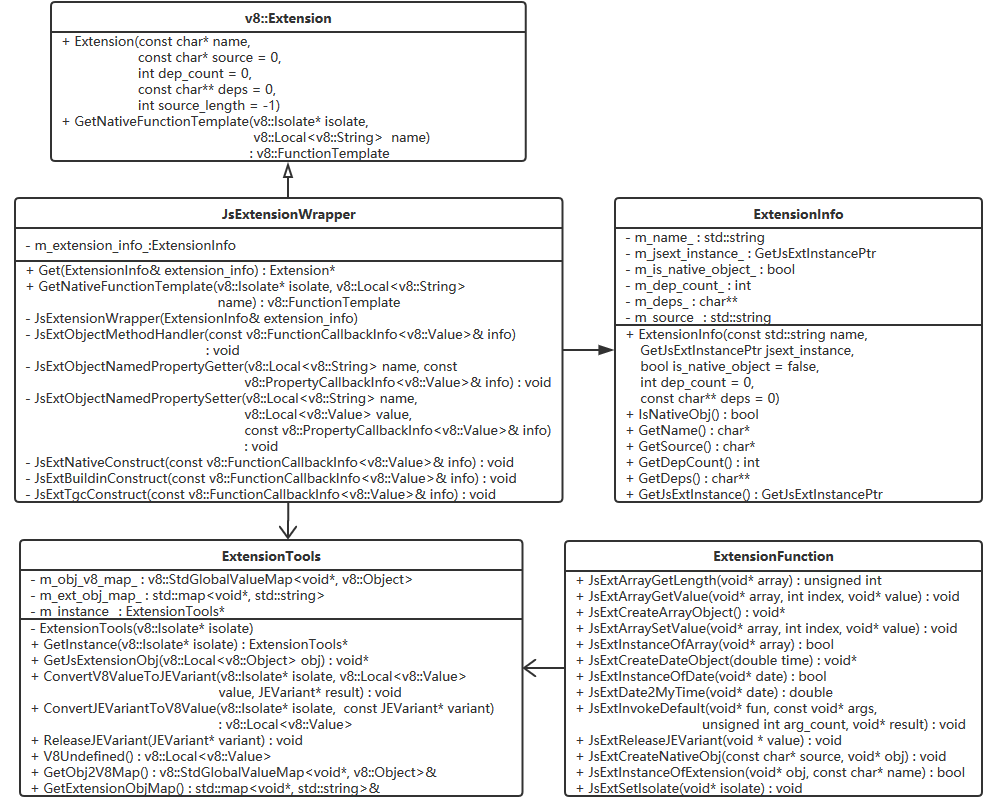
\includegraphics[width=\textwidth]{image/extension_framework/extension_framework_class.png} 
  \caption{extension framwork静态类图} \label{fig:extension_framework_class} 
\end{figure}

如第图~\ref{fig:extension_framework_class}所示:
v8扩展机制主要是继承v8内置的Extension类,通过重写其GetNativeFunctionTemplate方法来获取FunctionTemplate对象;
JsExtensionWrapper类主要就是封装创建出来的FunctionTemplate对象的一些特性,比如构造函数,属性拦截器,方法执行;
ExtensionInfo类主要记录了创建v8扩展所有需要的关键信息;ExtensionTools类主要是提供简易的函数,比如通过v8::Object类获取ExtensionBase对象,
将v8变量转换为扩展变量,将扩展变量转换为v8变量,释放扩展变量等;ExtensionFunction主要提供常用对外接口给js扩展调用。

\begin{figure}[H] 
  \centering 
  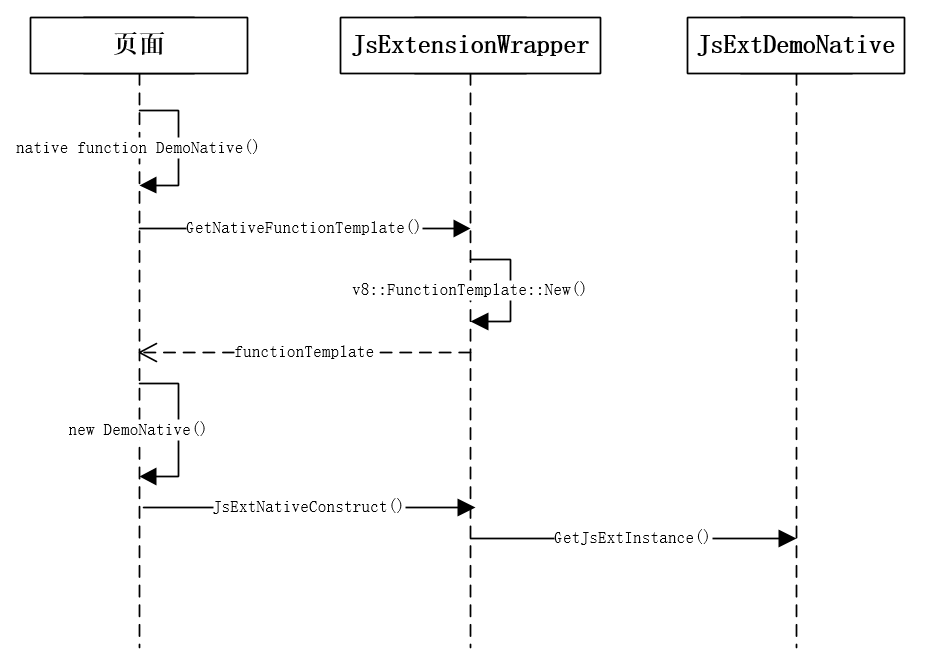
\includegraphics[width=\textwidth]{image/extension_framework/extension_construct_sequence.png} 
  \caption{js扩展对象创建时序图} \label{fig:extension_construct_sequence} 
\end{figure}

js扩展对象创建时序图如图~\ref{fig:extension_construct_sequence}所示:
\begin{itemize}
  \item 在页面加载时,v8::extension会注入页面代码native function DemoNative(),此时v8就会去创建DemoNative对应functionTemplate模板类。
  \item 当web开发人员在页面使用new DemoNative()时,functionTemplate模板类就会返回一个v8::Object实例对象给页面。
  \item 同理,针对内置对象,v8::extension会注入页面代码native function DemoBuildin()和var DemoBuildin = DemoBuildin()两段代码,
  此时由于DemoBuildin变量覆盖了DemoBuildin方法名,所以只能通过DemoBuildin执行对应方法和函数,不能再被new。
\end{itemize}

\begin{figure}[H] 
  \centering 
  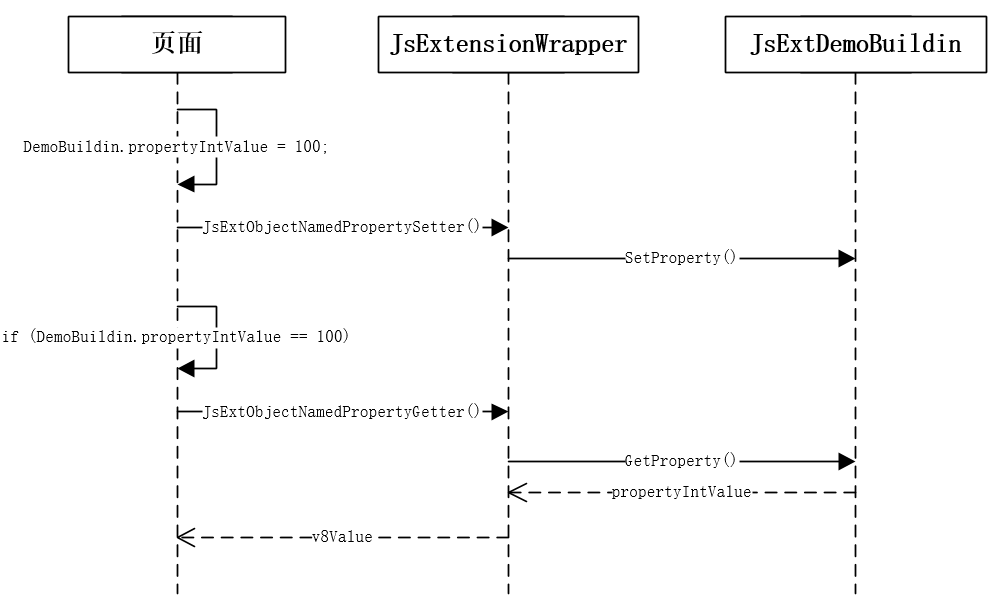
\includegraphics[width=\textwidth]{image/extension_framework/extension_property_sequence.png} 
  \caption{js扩展对象属性访问时序图} \label{fig:extension_property_sequence} 
\end{figure}

js扩展对象属性访问时序图如图~\ref{fig:extension_property_sequence}所示:
\begin{itemize}
  \item 由于在创建DemoBuildin对象时,对其ObjectTemplate模板类设置了拦截器特性,所以任何属性访问都会调用到拦截器的回调方法里。
\end{itemize}

\begin{figure}[H] 
  \centering 
  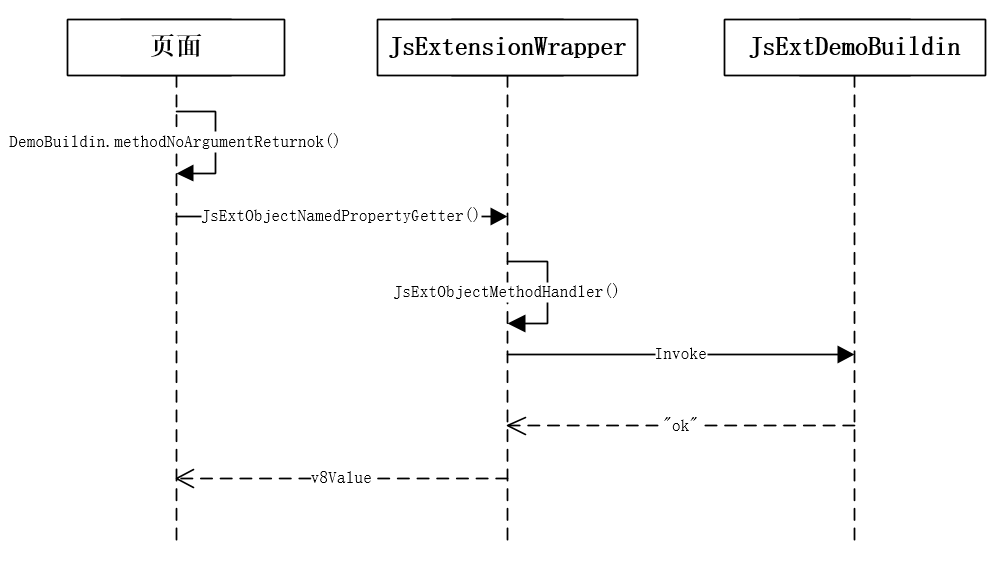
\includegraphics[width=\textwidth]{image/extension_framework/extension_function_sequence.png} 
  \caption{js扩展对象方法访问时序图} \label{fig:extension_function_sequence} 
\end{figure}

js扩展对象方法访问时序图如图~\ref{fig:extension_function_sequence}所示:
\begin{itemize}
  \item 同获取属性流程一致,当在拦截器回调函数里查询,如果属性没找到调用名,就去方法里找。
\end{itemize}

\section{Extension Framework垃圾回收机制}

对于内置对象,每次跳转页面,都会去调用其构造函数,此时回收机制的做法是先delete上个页面new出来的js扩展实例对象,再重新new一个js扩展实例对象,
然后绑定到v8 Object对象里。
\begin{spacing}{1.0}
\begin{lstlisting}[language={C++}]
void* delete_obj = ExtensionTools::GetJsExtensionObj(v8_obj);
  if (delete_obj) {
    ExtensionBase* ext_base = static_cast<ExtensionBase*>(delete_obj);
    delete ext_base;
    ext_base = NULL;
  }

  void* new_obj = NULL;
  extension_info->GetJsExtInstance()(NULL, 0, &new_obj);
  v8_obj->SetInternalField(ExtensionTools::JsExtBaseInternalField, v8::External::New(isolate, new_obj));
\end{lstlisting}
\end{spacing}

对于本地对象,每次创建对象时,我们会通过一个std::map保存js扩展实例对象指针以及name,当跳转页面,都会去调用tgc内置对象其构造函数,
将这个map里js扩展实例对象指针全部delete掉。
\begin{spacing}{1.0}
\begin{lstlisting}[language={C++}]
//在构造函数中将js扩展实例对象指针以及name保存到一个map中
void JsExtensionWrapper::JsExtNativeConstruct(const FunctionCallbackInfo<v8::Value>& info) {
  ...
  ExtensionTools* extension_tools = ExtensionTools::GetInstance(isolate);
  extension_tools->GetExtensionObjMap().insert(std::pair<void*, std::string>(new_obj, extension_info->GetName()));
  ...
}

//在tgc内置对象构造函数中将map中的js扩展实例对象指针全部delete掉
void JsExtensionWrapper::JsExtTgcConstruct(const FunctionCallbackInfo<v8::Value>& info) {
  ...
  ExtensionTools* extension_tools = ExtensionTools::GetInstance(isolate);
  std::map<void*, std::string>::iterator it;
  for (it = extension_tools->GetExtensionObjMap().begin(); it != extension_tools->GetExtensionObjMap().end(); it++) {
    ExtensionBase* ext_base = static_cast<ExtensionBase*>(it->first);
    if (ext_base) {
      delete ext_base;
      ext_base = NULL;
    }
  }
  ...
}
\end{lstlisting}
\end{spacing}



%---------------------------------------------------------------------

\ifx\withtbrowser\undefined
\else
\input{contents/extension_framework.tex}
\fi

\fi

\fi

\fi
